\documentclass[landscape,paperwidth=42in,paperheight=30in,margin=0.5in]{baposter}
\usepackage[utf8]{inputenc}
\usepackage{cmap}
\usepackage[T1]{fontenc}
\usepackage{beton}
\usepackage{eulervm}
\renewcommand{\sfdefault}{\rmdefault}
\usepackage{tikz}
\usetikzlibrary{positioning,arrows,automata,decorations.pathreplacing,decorations.text,decorations.markings,arrows,shapes,calc,fit}
\usepackage{caption}
\usepackage{subcaption}
\usepackage{multirow}
\usepackage{hhline}
\usepackage{graphicx}
\usepackage{amsmath}
\usepackage[noend]{algpseudocode}
\usepackage{relsize}
\usepackage{enumitem}

\setlist{nolistsep,leftmargin=*}

\begin{document}
\begin{poster}%
% Poster Options
{
    columns=3,
    % Show grid to help with alignment
    grid=false,
    % Column spacing
    colspacing=1em,
    % Format of textbox
    textborder=none,
    %textborder=rectangle,
    % Format of text header
    eyecatcher=false,
    headerborder=none,
    headerheight=0.1\textheight,
    headershape=rectangle,
    headershade=plain,
    headerfont=\Large\textsf, % Sans Serif
    boxshade=plain,
    %background=shade-tb,
    background=none,
    linewidth=2pt,
    boxColorOne=white,
    headerColorOne=white
}
% Eye Catcher
{}
% Title
{%
    \sf % Sans Serif
    %\bf % Serif
    \vspace{0.6em}
    Performance analysis of joins in reactive queries%
}
% Authors
{%
    \sf % Sans Serif
    %\bf % Serif
    Mitar Milutinović (mitar@tnode.com), Amy Pavel (amypavel@berkeley.edu)
}
% University logo
{%
    % TODO: Add Berkeley signature
    
\includegraphics[height=0.07\textheight]{ucseal_540_139}
}

%%%%%%%%%%%%%%%%%%%%%%%%%%%%%%%%%%%%%%%%%%%%%%%%%%%%%%%%%%%%%%%%%%%%%%%%%%%%%%
\headerbox{Motivation}{name=motivation,column=0,row=0}{
%%%%%%%%%%%%%%%%%%%%%%%%%%%%%%%%%%%%%%%%%%%%%%%%%%%%%%%%%%%%%%%%%%%%%%%%%%%%%%

NoSQL databases like MongoDB remove relations between documents and leave it to users to resolve relations on their own. Resolving relations on the client side results in round trip delays.
\\ \\
Modern web frameworks like Meteor provide an API to create reactive queries to the MongoDB: after initial query results, query is kept open and any update to the results set is streamed to the client. But if a query contains joins, constructing reactive queries by hand and resolving relations becomes hard. Moreover, consequence of multiple round trip delays accumulates.
\\ \\
PeerDB offers a way to embed useful fields from related documents and keep them updated, reducing read time on queries with joins, while allowing easy construction of reactive queries as well.

\vspace{1em}

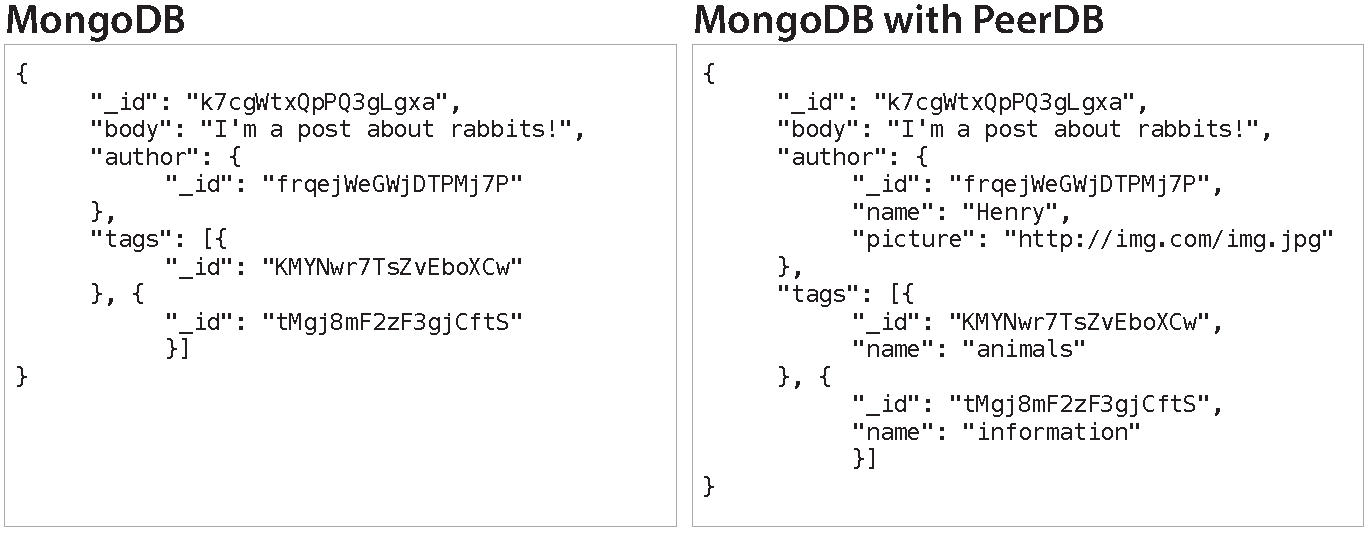
\includegraphics[width=\linewidth]{motivation}

\vspace{1em}

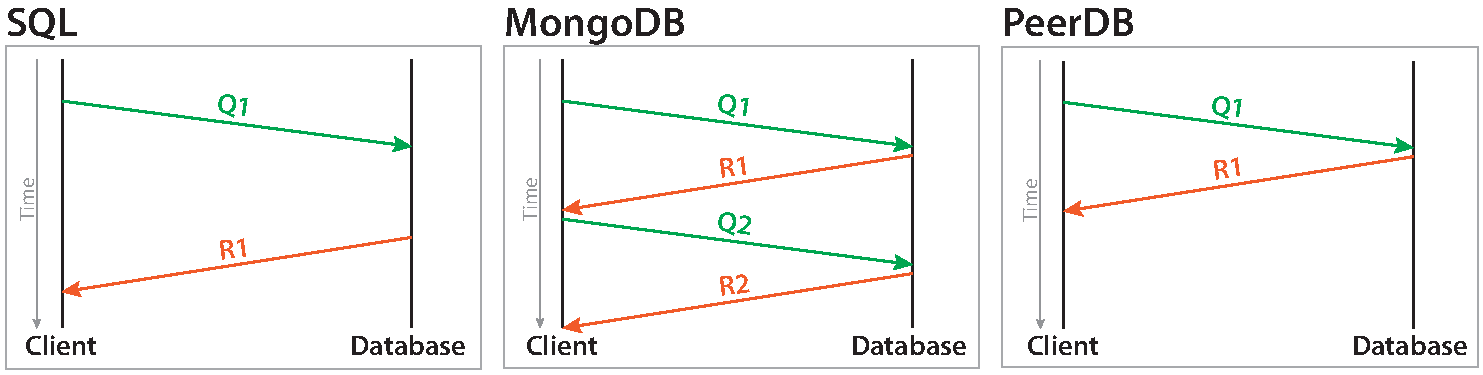
\includegraphics[width=\linewidth]{messages}

\vspace{1em}

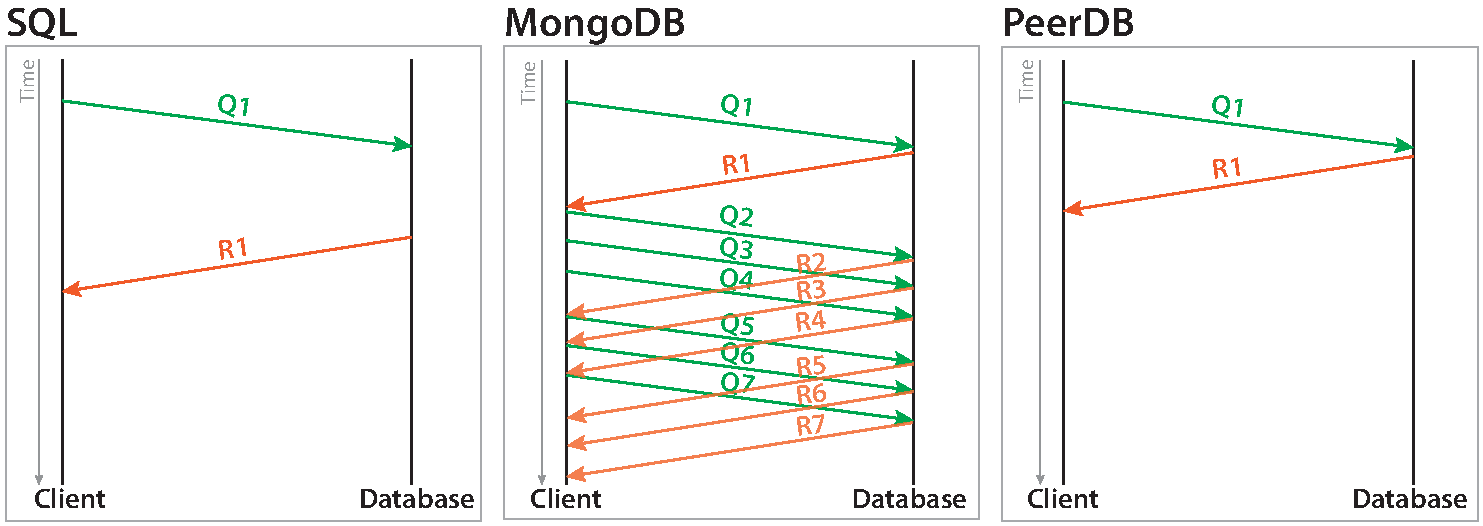
\includegraphics[width=\linewidth]{messages-many}

}

%%%%%%%%%%%%%%%%%%%%%%%%%%%%%%%%%%%%%%%%%%%%%%%%%%%%%%%%%%%%%%%%%%%%%%%%%%%%%%
\headerbox{Goals}{name=goals,column=1}{
%%%%%%%%%%%%%%%%%%%%%%%%%%%%%%%%%%%%%%%%%%%%%%%%%%%%%%%%%%%%%%%%%%%%%%%%%%%%%%

Evaluate PeerDB and recommend design guidelines for embedding fields. In particular, we will compare performance of the following variations using a blog application:
\begin{itemize}
\item PeerDB (high-level Meteor and low-level queries)
\item MongoDB (high-level Meteor and low-level queries)
\item Postgres (high-level Django and low-level queries)\\
\end{itemize}

\vspace{1em}

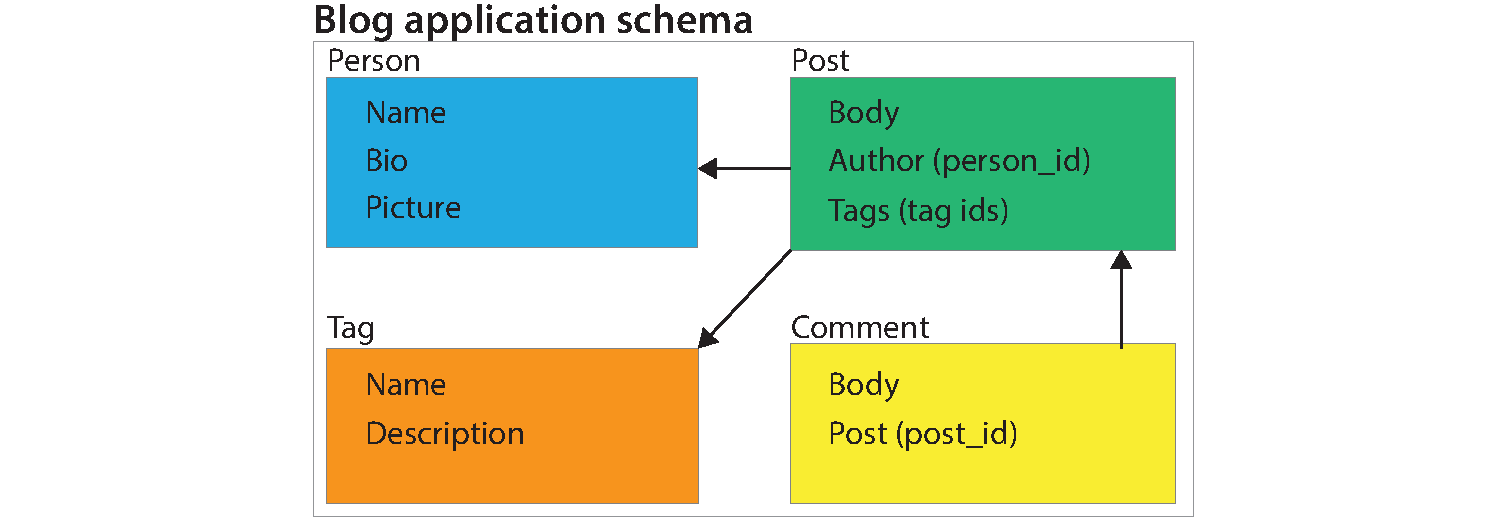
\includegraphics[width=\linewidth]{schema}

\vspace{1em}

We will offer design guidelines on when to use PeerDB embedded fields versus other methods by varying these parameters:
\begin{itemize}
\item Size of fields in related objects
\item Number of of objects
\item Number of database instances
\end{itemize}

}


%%%%%%%%%%%%%%%%%%%%%%%%%%%%%%%%%%%%%%%%%%%%%%%%%%%%%%%%%%%%%%%%%%%%%%%%%%%%%%
\headerbox{Comparison results}{name=comparison,column=1, below=goals}{
%%%%%%%%%%%%%%%%%%%%%%%%%%%%%%%%%%%%%%%%%%%%%%%%%%%%%%%%%%%%%%%%%%%%%%%%%%%%%%

We found that high performance reads of PeerDB come at the expense of slow writes (figure to the right). Based on our evaluation we recommend using postgres for write-heavy applications. 

\vspace{1em}

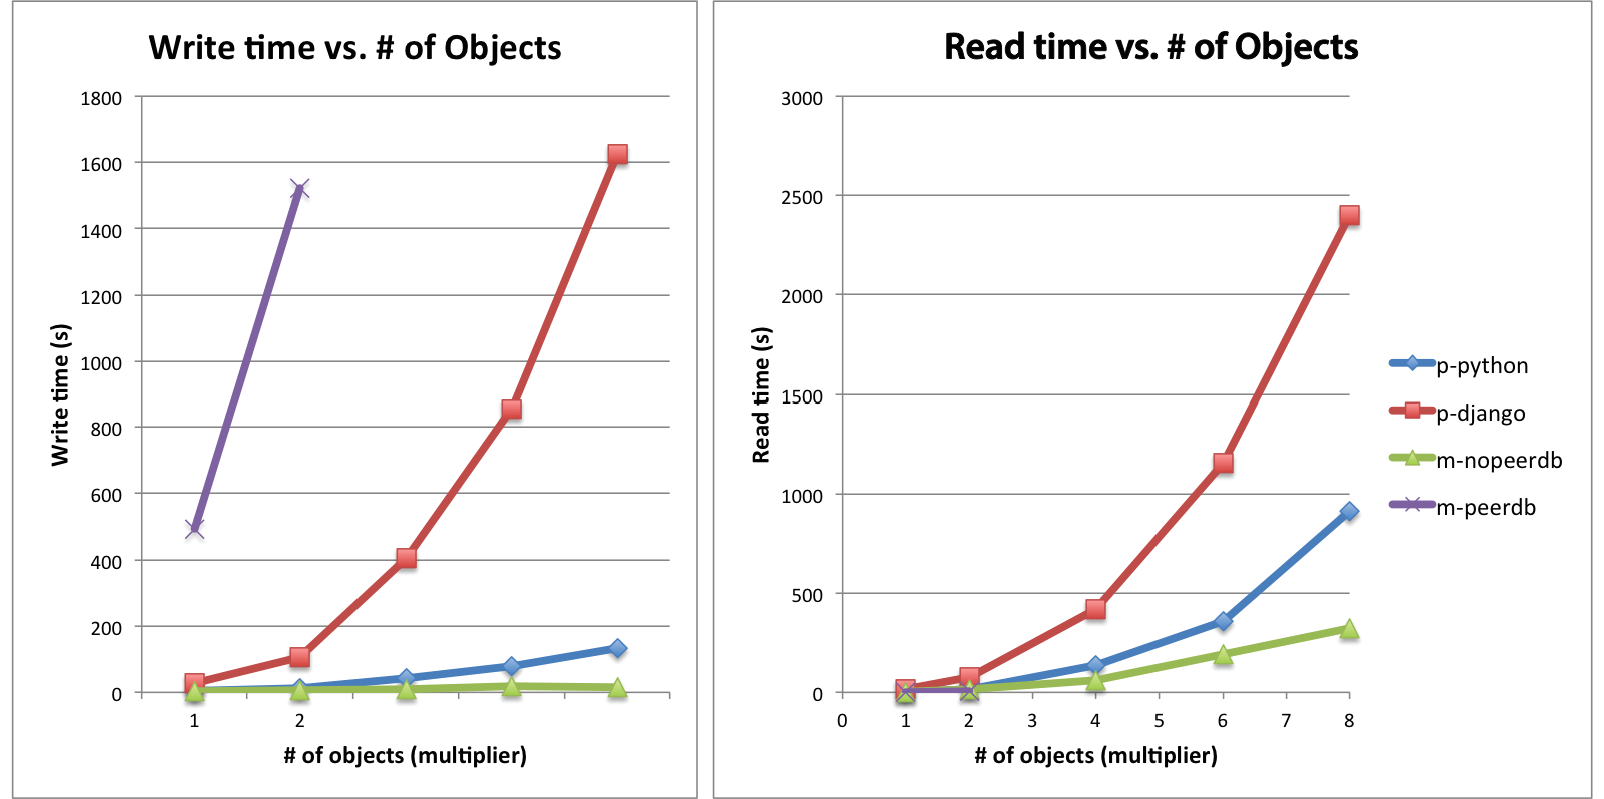
\includegraphics[width=\linewidth]{graphs}

}

%%%%%%%%%%%%%%%%%%%%%%%%%%%%%%%%%%%%%%%%%%%%%%%%%%%%%%%%%%%%%%%%%%%%%%%%%%%%%%
\headerbox{Design guidelines}{name=design,column=2}{
%%%%%%%%%%%%%%%%%%%%%%%%%%%%%%%%%%%%%%%%%%%%%%%%%%%%%%%%%%%%%%%%%%%%%%%%%%%%%%

Based on our evaluation and use of PeerDB in PeerLibrary we came up with the following design guidelines for picking fields to embed. These design considerations can be automated or handled during schema specification.
\\ 
\begin{itemize}
\item Fields to embed are small in size
\item Values of all embedded fields are shared across all queries
\item Reads on documents using embedded fields are much more common than writes
\end{itemize}


}

%%%%%%%%%%%%%%%%%%%%%%%%%%%%%%%%%%%%%%%%%%%%%%%%%%%%%%%%%%%%%%%%%%%%%%%%%%%%%%
\headerbox{Reactive queries with joins}{name=reactive,column=2,below=design}{
%%%%%%%%%%%%%%%%%%%%%%%%%%%%%%%%%%%%%%%%%%%%%%%%%%%%%%%%%%%%%%%%%%%%%%%%%%%%%%

In addition to making static queries to evaluate PeerDB performance we evaluated reactive queries with joins as well.

\vspace{1em}

}

%%%%%%%%%%%%%%%%%%%%%%%%%%%%%%%%%%%%%%%%%%%%%%%%%%%%%%%%%%%%%%%%%%%%%%%%%%%%%%
\headerbox{Related work}{name=related,column=2,below=reactive}{
%%%%%%%%%%%%%%%%%%%%%%%%%%%%%%%%%%%%%%%%%%%%%%%%%%%%%%%%%%%%%%%%%%%%%%%%%%%%%%

\begin{itemize}
\item Materialized views
\item Column stores and database cracking
\item Customizing NoSQL databases
\end{itemize}

}

%%%%%%%%%%%%%%%%%%%%%%%%%%%%%%%%%%%%%%%%%%%%%%%%%%%%%%%%%%%%%%%%%%
\headerbox{Github links}{name=github,column=2,below=related}{
%%%%%%%%%%%%%%%%%%%%%%%%%%%%%%%%%%%%%%%%%%%%%%%%%%%%%%%%%%%%%%%%%%%%%%%%%%%%%%

PeerDB: github.com/peerlibrary/meteor-peerdb \\
Benchmarking: github.com/mitar/peerdb-benchmark

}

\end{poster}
\end{document}
